% задание и сама лабораторная работа
% Для листинга кода:
\lstset{ %
	language=C,                % Язык программирования                % где поставить нумерацию строк (слева\справа)
	numberstyle=\tiny,           % размер шрифта для номеров строк
	stepnumber=1,                   % размер шага между двумя номерами строк
	numbersep=5pt,                % как далеко отстоят номера строк от подсвечиваемого кода
	showspaces=false,            % показывать или нет пробелы специальными отступами
	showstringspaces=false,      % показывать или нет пробелы в строках
	showtabs=false,             % показывать или нет табуляцию в строках
	tabsize=2,                 % размер табуляции по умолчанию равен 2 пробелам
	captionpos=t,              % позиция заголовка вверху [t] или внизу [b] 
	breaklines=true,           % автоматически переносить строки (да\нет)
	breakatwhitespace=false,       
	frame=single,                    % Добавить рамку
	basicstyle=\small,
	escapebegin=\begin{russian}\commentfont,
		escapeend=\end{russian},
	literate={Ö}{{\"O}}1
	{Ä}{{\"A}}1
	{Ü}{{\"U}}1
	{ß}{{\ss}}1
	{ü}{{\"u}}1
	{ä}{{\"a}}1
	{ö}{{\"o}}1
	{~}{{\textasciitilde}}1
	{а}{{\selectfont\char224}}1
	{б}{{\selectfont\char225}}1
	{в}{{\selectfont\char226}}1
	{г}{{\selectfont\char227}}1
	{д}{{\selectfont\char228}}1
	{е}{{\selectfont\char229}}1
	{ё}{{\"e}}1
	{ж}{{\selectfont\char230}}1
	{з}{{\selectfont\char231}}1
	{и}{{\selectfont\char232}}1
	{й}{{\selectfont\char233}}1
	{к}{{\selectfont\char234}}1
	{л}{{\selectfont\char235}}1
	{м}{{\selectfont\char236}}1
	{н}{{\selectfont\char237}}1
	{о}{{\selectfont\char238}}1
	{п}{{\selectfont\char239}}1
	{р}{{\selectfont\char240}}1
	{с}{{\selectfont\char241}}1
	{т}{{\selectfont\char242}}1
	{у}{{\selectfont\char243}}1
	{ф}{{\selectfont\char244}}1
	{х}{{\selectfont\char245}}1
	{ц}{{\selectfont\char246}}1
	{ч}{{\selectfont\char247}}1
	{ш}{{\selectfont\char248}}1
	{щ}{{\selectfont\char249}}1
	{ъ}{{\selectfont\char250}}1
	{ы}{{\selectfont\char251}}1
	{ь}{{\selectfont\char252}}1
	{э}{{\selectfont\char253}}1
	{ю}{{\selectfont\char254}}1
	{я}{{\selectfont\char255}}1
	{А}{{\selectfont\char192}}1
	{Б}{{\selectfont\char193}}1
	{В}{{\selectfont\char194}}1
	{Г}{{\selectfont\char195}}1
	{Д}{{\selectfont\char196}}1
	{Е}{{\selectfont\char197}}1
	{Ё}{{\"E}}1
	{Ж}{{\selectfont\char198}}1
	{З}{{\selectfont\char199}}1
	{И}{{\selectfont\char200}}1
	{Й}{{\selectfont\char201}}1
	{К}{{\selectfont\char202}}1
	{Л}{{\selectfont\char203}}1
	{М}{{\selectfont\char204}}1
	{Н}{{\selectfont\char205}}1
	{О}{{\selectfont\char206}}1
	{П}{{\selectfont\char207}}1
	{Р}{{\selectfont\char208}}1
	{С}{{\selectfont\char209}}1
	{Т}{{\selectfont\char210}}1
	{У}{{\selectfont\char211}}1
	{Ф}{{\selectfont\char212}}1
	{Х}{{\selectfont\char213}}1
	{Ц}{{\selectfont\char214}}1
	{Ч}{{\selectfont\char215}}1
	{Ш}{{\selectfont\char216}}1
	{Щ}{{\selectfont\char217}}1
	{Ъ}{{\selectfont\char218}}1
	{Ы}{{\selectfont\char219}}1
	{Ь}{{\selectfont\char220}}1
	{Э}{{\selectfont\char221}}1
	{Ю}{{\selectfont\char222}}1
	{Я}{{\selectfont\char223}}1
	{і}{{\selectfont\char105}}1
	{ї}{{\selectfont\char168}}1
	{є}{{\selectfont\char185}}1
	{ґ}{{\selectfont\char160}}1
	{І}{{\selectfont\char73}}1
	{Ї}{{\selectfont\char136}}1
	{Є}{{\selectfont\char153}}1
	{Ґ}{{\selectfont\char128}}1
}

\newpage
\section*{Задание 1}
\addcontentsline{toc}{section}{\tocsecindent{Задание 1}}
\subsection*{Постановка задачи}
\addcontentsline{toc}{subsection}{\tocsecindent{Постановка задачи}}
Реализовать загружаемый модуль ядра, выводящий информацию о процессах.


\subsection*{Листинг кода}
\addcontentsline{toc}{subsection}{\tocsecindent{Листинг кода}}

\begin{lstlisting}[language=c,caption=Листинг кода загружаемого модуль ядра для задания 1]
#include <linux/init.h>
#include <linux/module.h>
#include <linux/kernel.h>
#include <linux/sched/task.h>
#include <linux/sched/signal.h>

MODULE_LICENSE("GPL");
MODULE_AUTHOR("Furdik");
MODULE_DESCRIPTION("Lab3");

static int __init my_module_init(void)
{
	printk(KERN_INFO "MODULE1: loaded!\n");

	struct task_struct *task = &init_task;
	do
	{
		printk(KERN_INFO "MODULE1: process: %s - %d, parent: %s - %d\n",
				task->comm, task->pid, task->parent->comm, task->parent->pid);
	}
	while ((task = next_task(task)) != &init_task);

	printk(KERN_INFO "MODULE1: current: %s - %d, parent: %s - %d",
			current->comm, current->pid, current->parent->comm, current->parent->pid);
		
	return 0;
}

static void __exit my_module_exit(void)
{
	printk(KERN_INFO "MODULE1: unloaded\n");
}

module_init(my_module_init);
module_exit(my_module_exit);
\end{lstlisting}
\newpage
\section*{Результат работы}
\addcontentsline{toc}{subsection}{\tocsecindent{Результат работы}}
1. Скомпилируем модуль ядра и загрузим его, проверив успешную загрузку с помозью списка загруженных модулей ядра.
\begin{figure}[h!]
\center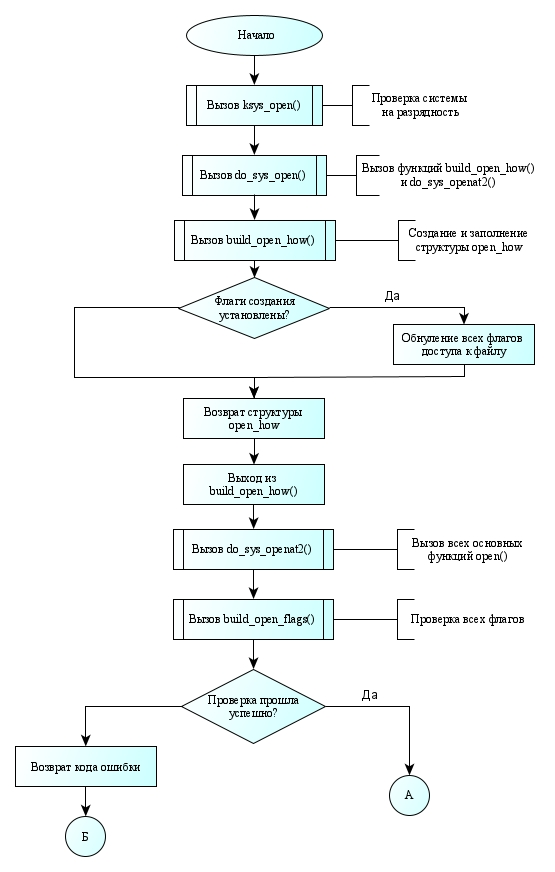
\includegraphics[scale=1]{1.jpg}
\end{figure}
\begin{figure}[h!]
\center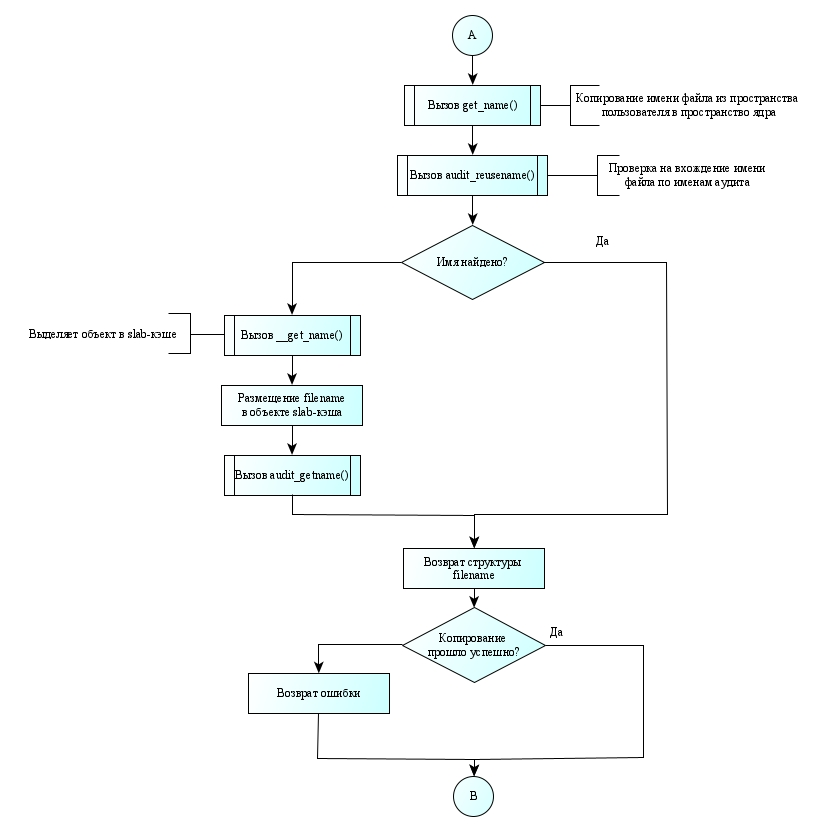
\includegraphics[scale=1]{2.jpg}
\end{figure}
\newline 2. Просмотрим сообщения буфера ядра, записанные в логи:
\begin{figure}[h!]
\center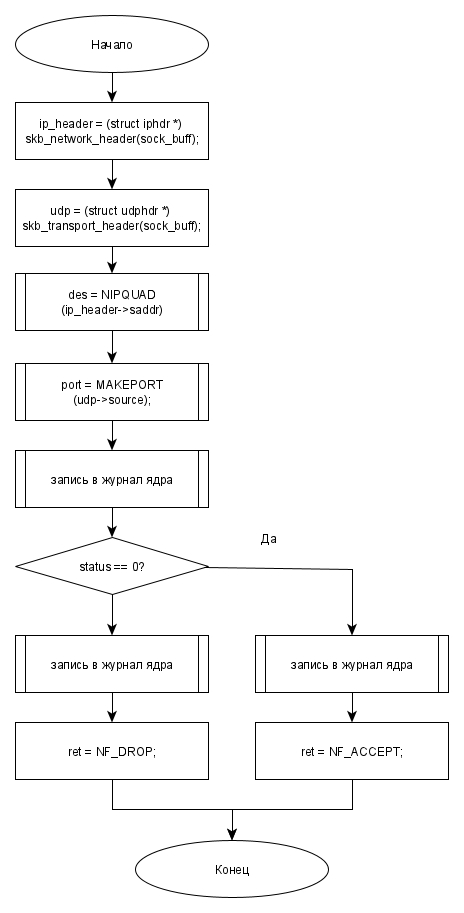
\includegraphics[scale=1]{3.jpg}
\end{figure}
\newpage
\begin{figure}[h!]
	\center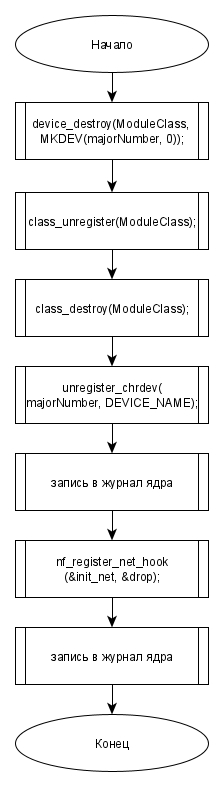
\includegraphics[scale=1]{4.jpg}
\end{figure}
3. Выгрузим модуль:
\begin{figure}[h!]
\center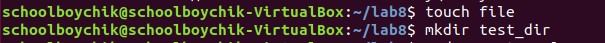
\includegraphics[scale=1]{5.jpg}
\end{figure}
\newpage
\section*{Задание 2}
\addcontentsline{toc}{section}{\tocsecindent{Задание 2}}
\subsection*{Постановка задачи}
\addcontentsline{toc}{subsection}{\tocsecindent{Постановка задачи}}
Реализовать три загружаемых модуля ядра:
\begin{enumerate}

	\item вызываемый модуль md1;
	\item вызывающий модуль md2;
	\item «отладочный» модуль md3.
\end{enumerate}



\subsection*{Листинг кода}
\addcontentsline{toc}{subsection}{\tocsecindent{Листинг кода}}

\begin{lstlisting}[language=c,caption=Листинг кода вызываемого модуля md1]
#include <linux/init.h>
#include <linux/module.h>
#include "md.h"

MODULE_LICENSE("GPL");
MODULE_AUTHOR("Furdik");
MODULE_DESCRIPTION("Lab3");

char* md1_str_data = "Привет из модуля 1!";
int md1_int_data = 111;

extern char* md1_get_str(int n)
{
	printk(KERN_INFO "MODULE1: md1_get_str(%d) called\n", n);
	switch (n)
	{
		case 1:
			return "Привет!";
			break;
		case 2:
			return "Пока!";
			break;
		default:
			return "Передайте 1 для приветствия или 2 для прощания";
			break;
	}
}

extern int md1_factorial(int n)
{
	printk(KERN_INFO "MODULE1: md1_factorial(%d) called\n", n);

	int i, answer = 1;

	if (n <= 0)
		return 0;

	for (i = 2; i <= n; i++)
		answer *= i;

	return answer;
}

EXPORT_SYMBOL(md1_str_data);
EXPORT_SYMBOL(md1_int_data);
EXPORT_SYMBOL(md1_get_str);
EXPORT_SYMBOL(md1_factorial);

static int __init my_module_init(void)
{
	printk(KERN_INFO "MODULE1: loaded\n");
	return 0;
}

static void __exit my_module_exit(void)
{
	printk(KERN_INFO "MODULE1: unloaded\n");
}

module_init(my_module_init);
module_exit(my_module_exit);

\end{lstlisting}

\begin{lstlisting}[language=c,caption=Листинг кода вызывающего модуля md2]
#include <linux/init.h>
#include <linux/module.h>
#include "md.h"

MODULE_LICENSE("GPL");
MODULE_AUTHOR("Furdik");
MODULE_DESCRIPTION("Lab3");

static int __init my_module_init(void)
{
	printk(KERN_INFO "MODULE2: loaded\n");
	printk(KERN_INFO "MODULE2: Число экспортированное из md1 : %d\n", md1_int_data);
	printk(KERN_INFO "MODULE2: Строка экспортированная из md1 : %s\n", md1_str_data);
	printk(KERN_INFO "MODULE2: Результат работы функции md1_get_str(10) : %s\n", md1_get_str(10));
	printk(KERN_INFO "MODULE2: Результат работы функции md1_get_str(1) : %s\n", md1_get_str(1));
	printk(KERN_INFO "MODULE2: Результат работы функции md1_get_str(2) : %s\n", md1_get_str(2));
	printk(KERN_INFO "MODULE2: Результат работы функции md1_factorial(10) : %d\n", md1_factorial(10));
	return 0;
}

static void __exit my_module_exit(void)
{
	printk(KERN_INFO "MODULE2: unloaded\n");
}

module_init(my_module_init);
module_exit(my_module_exit);


\end{lstlisting}
\begin{lstlisting}[language=c,caption=Листинг кода "отладочного" модуля md3]
#include <linux/init.h>
#include <linux/module.h>
#include "md.h"

MODULE_LICENSE("GPL");
MODULE_AUTHOR("Furdik");
MODULE_DESCRIPTION("Lab3");

static int __init my_module_init(void)
{
	printk(KERN_INFO "MODULE3: loaded\n");
	printk(KERN_INFO "MODULE3: Число экспортированное из md1 : %d\n", md1_int_data);
	printk(KERN_INFO "MODULE3: Строка экспортированная из md1 : %s\n", md1_str_data);
	printk(KERN_INFO "MODULE3: Результат работы функции md1_get_str(2) : %s\n", md1_get_str(10));
	printk(KERN_INFO "MODULE3: Результат работы функции md1_get_str(0) : %s\n", md1_get_str(1));
	printk(KERN_INFO "MODULE3: Результат работы функции md1_get_str(1) : %s\n", md1_get_str(2));
	printk(KERN_INFO "MODULE3: Результат работы функции md1_factorial(4) : %d\n", md1_factorial(10));
	return -1;
}

module_init(my_module_init);


\end{lstlisting}
\section*{Результат работы}
\addcontentsline{toc}{subsection}{\tocsecindent{Результат работы}}
1. Скомпилируем модули ядра и загрузим первые два из них, проверив успешную загрузку с помощью списка загруженных модулей ядра.
\begin{figure}[h!]
	\center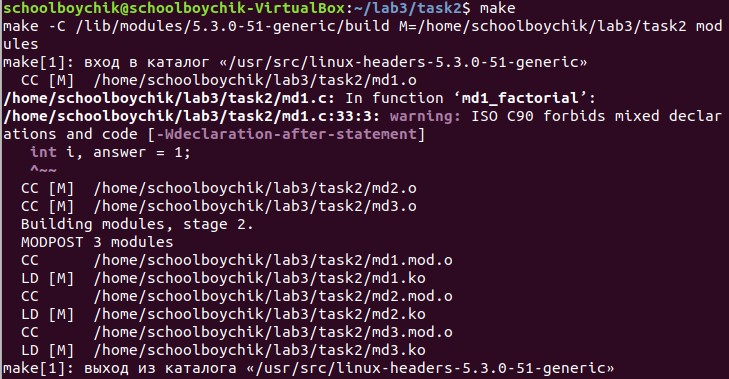
\includegraphics[scale=1]{6.jpg}
\end{figure}
\begin{figure}[h!]
	\center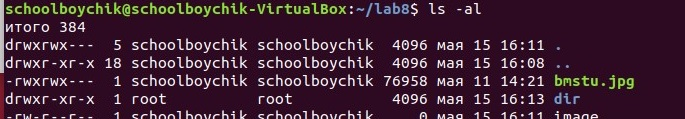
\includegraphics[scale=1]{12.jpg}
\end{figure}
\newline Как видно из вывода команды lsmod, модуль md1 используется модулем md2. Следовательно, важен порядок загрузки/выгрузки: загружать нужно сначала md1, затем md2; выгрузка должна происходить в обратном порядке.
\begin{figure}[h!]
	\center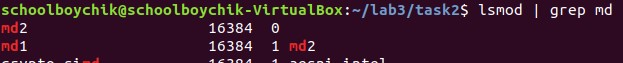
\includegraphics[scale=1]{11.jpg}
\end{figure}
\newline Пример ошибочного и правильного порядков выгрузки:
\begin{figure}[h!]
	\center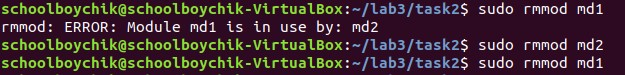
\includegraphics[scale=1]{14.jpg}
\end{figure}
\newline 2. Просмотрим сообщения буфера ядра, записанные в логи:
\begin{figure}[h!]
	\center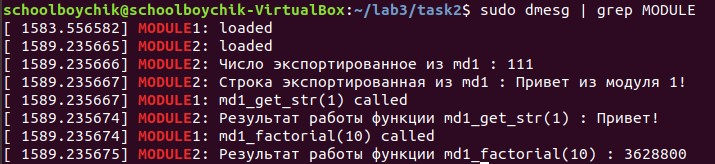
\includegraphics[scale=1]{16.jpg}
\end{figure}
\newline 3. Выгрузим модули ядра в правильном порядке:
\begin{figure}[h!]
	\center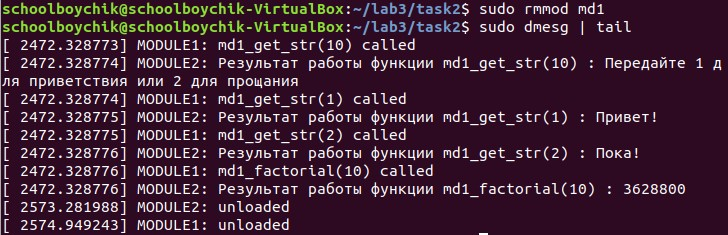
\includegraphics[scale=1]{8.jpg}
\end{figure}
\newline 4. Теперь загрузим вызываемый и "отладочный" модули, последний из которых преднамеренно возвращает ненулевое значение, что означает ошибку инициализации модуля.
\begin{figure}[h!]
	\center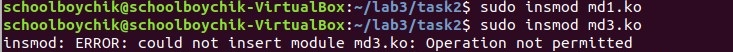
\includegraphics[scale=1]{9.jpg}
\end{figure}
\newpage
\begin{figure}[h!]
	\center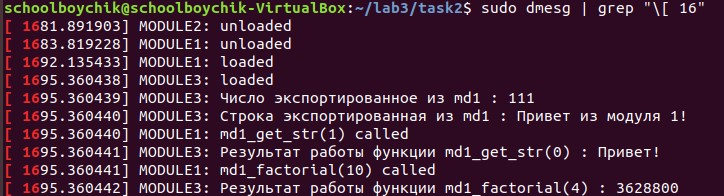
\includegraphics[scale=1]{17.jpg}
\end{figure}
"Отладочный" модуль не будет подгружен к ядру, однако это станет известно уже после выполнения кода инициализирующей функции модуля в пространстве ядра:
\begin{figure}[h!]
	\center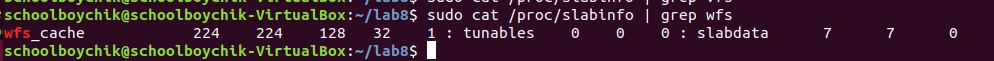
\includegraphics[scale=1]{10.jpg}
\end{figure}
\newline 5. Продемонстриуем ошибочную ситуацию. В данных модулях продемострирована работа экспортируемых данных и функций: модуль md1 экспортирует переменные md1\_str\_data и md1\_int\_data, которые импортируют модули md2 и md3. Поскольку md2 и md3 импортируют данные из модуля md1, то они не могут быть загружены до загрузки модуля md1: \begin{figure}[h!]
	\center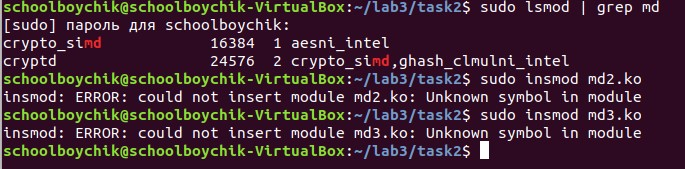
\includegraphics[scale=1]{15.jpg}
\end{figure}


